\documentclass[aspectratio=169,14pt]{beamer}
\usetheme[titleformat=regular%
,numbering=fraction% use slide numbers
]{metropolis}
\usepackage{appendixnumberbeamer} % separate appendix
\usepackage[citestyle=authortitle-icomp]{biblatex}
\setbeamerfont{footnote}{size=\tiny}
\addbibresource{mae.bib}

% multimedia in beamer presentations
\usepackage{multimedia}

% adding some better facilities to latex such as proper booleans
\usepackage{etoolbox}

% Unicode math symbols for XeLaTeX
\usepackage{mathrsfs}

% standard math packages
\usepackage{amssymb}
\usepackage{amsthm}
\usepackage{amsmath}
\usepackage{amstext}
\usepackage{mathabx}
\usepackage{stmaryrd}
% math tools for amsmath
\usepackage{mathtools}

\usepackage{proof}

\usepackage{listings}
\usepackage{xcolor}

% subfigures, subfloats
\usepackage{subcaption}

% for multiinclude
\usepackage{xmpmulti}

% tikz & friends

\usepackage{galois}
\usepackage{tikz}
\usetikzlibrary{fit,calc,shapes,arrows.meta,patterns,backgrounds}
\usetikzlibrary{decorations.pathmorphing}
\usetikzlibrary{cd}
\usepackage[beamer]{hf-tikz}

\newcommand{\tikzmark}[1]{%
  \tikz[overlay,remember picture,baseline] \node [anchor=base] (#1) {};}

\newenvironment{tightcenter}{%
  \setlength\topsep{0pt}
  \setlength\parskip{0pt}
  \begin{center}
}{%
  \end{center}
}

% new colors
\definecolor{lightblue}{RGB}{217,220,253}
\definecolor{lightred}{RGB}{251,216,218}

\DeclareMathOperator{\pw}{\mathcal{P}} % powerset
\newcommand{\fset}[1]{\mathsf{#1}}
\newcommand{\nats}{\mathbb{N}}
\newcommand{\zahlen}{\mathbb{Z}}
\newcommand{\bools}{\mathbb{B}}
\newcommand{\Set}[1]{\left\{#1\right\}}
\newcommand{\true}{\kw{true}}
\newcommand{\false}{\kw{false}}
\newcommand{\sidenote}[1]{\hfill\quad \textsf{#1}}

\newcommand{\disunion}{+}

% named set
\newcommand{\ns}[1]{\mathit{#1}}
% function
\newcommand{\fn}[1]{\mathrm{#1}}
% "vector of"
\newcommand{\vo}[1]{\overrightarrow{#1}}
% "set of"
\newcommand{\setOf}[1]{\overline{#1}}
% syntactic tag
\newcommand{\sTag}[2]{\textsf{\textbf{#1}}\,#2}
% keyword
\newcommand{\kw}[1]{\texttt{#1}}
% usual suspects
\newcommand{\State}{\ns{State}}
\newcommand{\Value}{\ns{Value}}
\newcommand{\Stmt}{\ns{Stmt}}
\newcommand{\Env}{\ns{Env}}
\newcommand{\Store}{\ns{Store}}
\newcommand{\Kont}{\ns{Kont}}
% syntactic domains
\newcommand{\Exp}{\ns{Exp}}
\newcommand{\Var}{\ns{Var}}
\newcommand{\Addr}{\ns{Addr}}
% put a value to a pointer
\newcommand{\update}{\leftarrow}

% ebnf
\newcommand{\eDEF}{\,::=\;}
\newcommand{\eOR}{\;\vert\;}

\newcommand{\widen}{\nabla}

% \newcommand{\|}{\,\vert\,}

\newcommand{\todo}[1]{\iftoggle{TODO}{\textcolor{red}{TODO: #1}}{}}
% ceiling and floor symbols
\DeclarePairedDelimiter\ceil{\lceil}{\rceil}
\DeclarePairedDelimiter\floor{\lfloor}{\rfloor}

% big O notation
\DeclareMathOperator{\bigO}{O}

% fixed points
\DeclareMathOperator{\lfp}{lfp}

% print both years for bibliography
\renewbibmacro*{cite:labelyear+extrayear}{%
\iffieldundef{labelyear}
{}
{\printtext[bibhyperref]{%
\iffieldundef{origyear}{}{\printfield{origyear}\addslash}%   <--- added
\printfield{labelyear}%
\printfield{extrayear}}}}

\renewbibmacro*{date+extrayear}{%
\iffieldundef{year}
{}
{\printtext[parens]{%
\iffieldundef{origyear}{}{\printfield{origyear}\addslash}%  <--- added
\printdateextra}}}

% overlay an image
\def\Put(#1,#2)#3{\leavevmode\makebox(0,0){\put(#1,#2){#3}}}

% text over symbols nicely, requires amsmath for overset
\newcommand\textoverop[2]{\mathrel{\overset{\makebox[0pt]{\mbox{\normalfont\tiny\sffamily #1}}}{#2}}}

% special arrows
\newcommand\monarrow{\textoverop{mon}{\rightarrow}}

% theorems
\newtheorem{thm}{Theorem}
\newtheorem{eg}{Example}

\newcommand{\abscolor}[1]{\textcolor{mLightBrown}{#1}}
\newcommand{\concolor}[1]{\textcolor{mLightGreen}{#1}}
\newcommand{\abst}[1]{#1^{\#}}

\newcommand{\step}{\rightsquigarrow}

% listings setup
\lstset{basicstyle=\tiny\ttfamily,columns=fixed}

%%% Local Variables:
%%% mode: latex
%%% TeX-master: "main"
%%% TeX-engine: xetex
%%% End:


\title[Major Area Exam]{Abstract Interpretation of Low-level Programs}
\subtitle{Major Area Exam}
\date{January 23, 2018}
\author{Mehmet Emre}
\institute[UCSB]{
  \normalsize
  {\large \bfseries Committee:}\\
  Ben Hardekopf (\,$\vcenter{\hbox{
\includegraphics[height=1em]{chair/file.eps}}}$) \quad
  Tevfik Bultan \quad
  Chandra Krintz
}
\titlegraphic{\hfill
\includegraphics[width=1.5cm]{ucsbseal_cmyk.pdf}}

\begin{document}
\maketitle

\begin{frame}{Outline}
  \small
  \vspace{0.5em}
  \tableofcontents
\end{frame}

\section{Introduction}
\begin{frame}{What is low-level software? Why should we analyze it?}
Low-level software:
\begin{itemize}
\item Interacts with intricate APIs (drivers, kernel modules, databases)
\item Require preserving subtle invariants (above, control software)
\item Have heavy reliability requirements
\begin{itemize}
\item with unpleasant consequences % : BSoD, data loss, Arianne~5, Heartbleed, Patriot missile
\end{itemize}
\end{itemize}

\end{frame}

{ % all template changes are local to this group.
    \setbeamertemplate{navigation symbols}{}
    \begin{frame}[plain]
        \begin{tikzpicture}[remember picture,overlay]
            \node[at=(current page.center)] {
                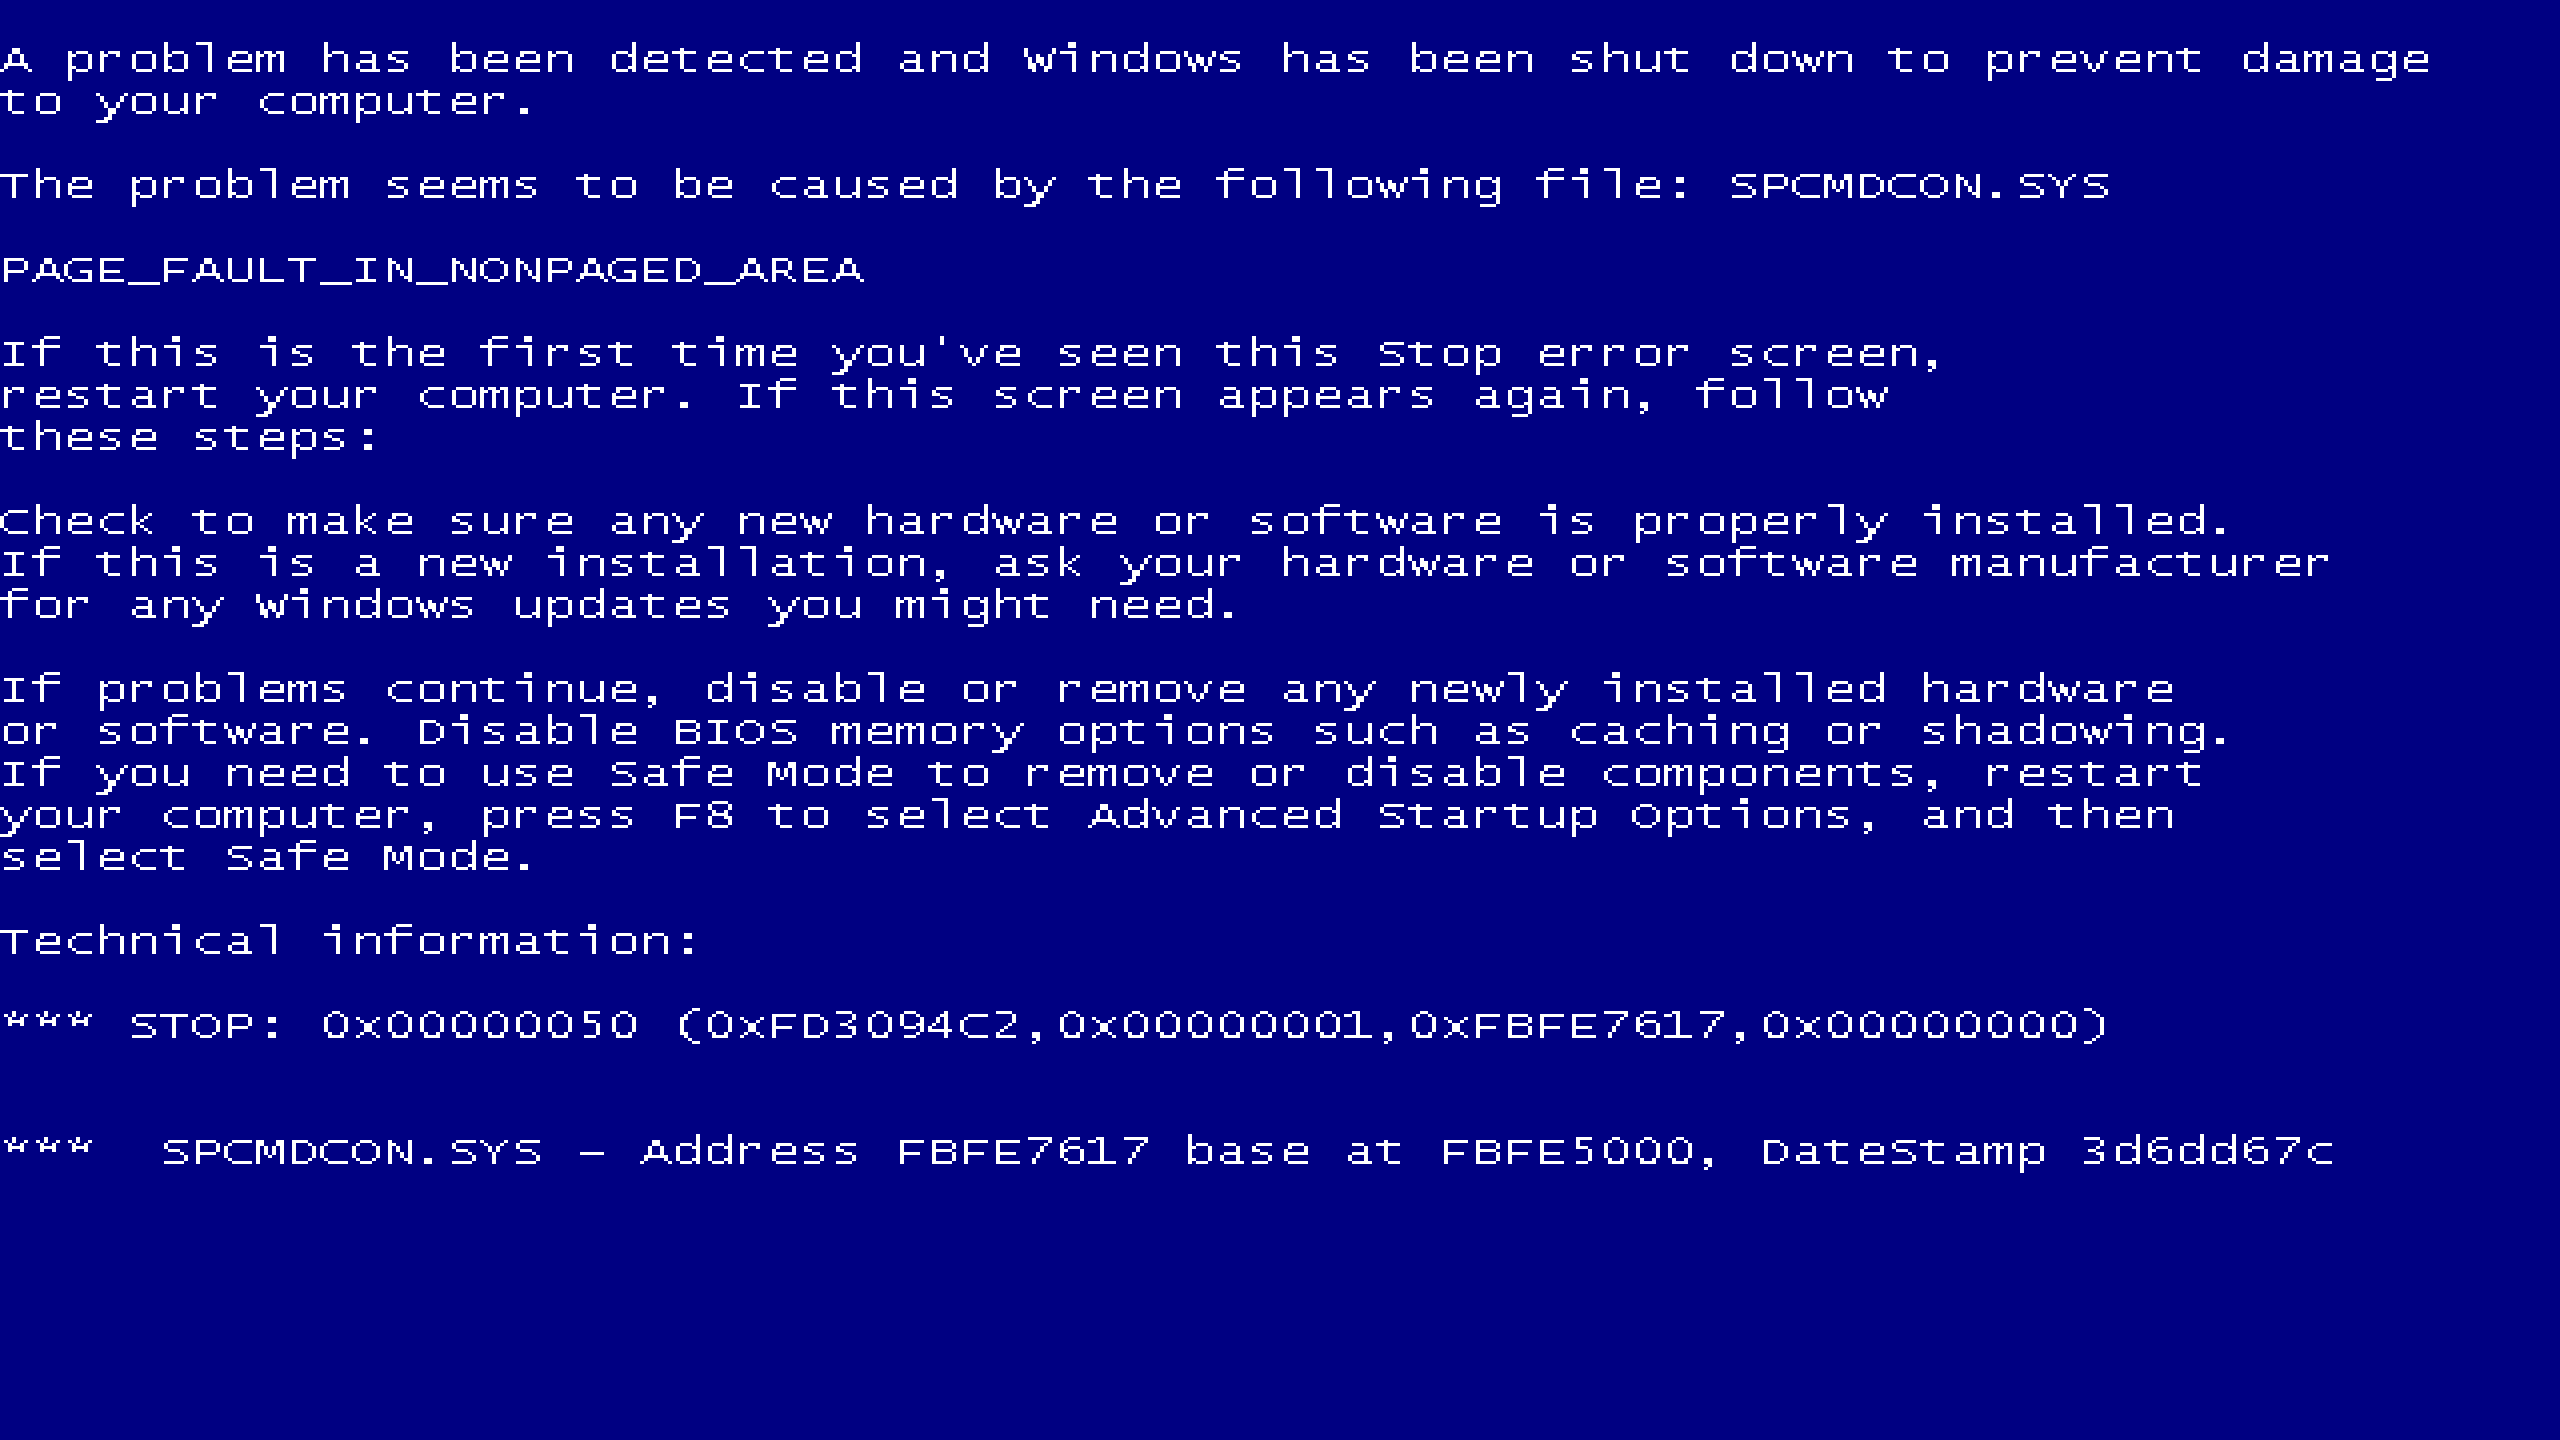
\includegraphics[width=\paperwidth]{material/bsod_resized.png}
            };
          \end{tikzpicture} \pause

          \Put(10,10){
\includegraphics[width=0.4\textwidth]{material/heartbleed.pdf}}\pause
          \Put(180,200){
\includegraphics[width=0.4\textwidth]{material/formal-verification-as-a-sinking-airplane.png}}\pause
          \Put(210,-50){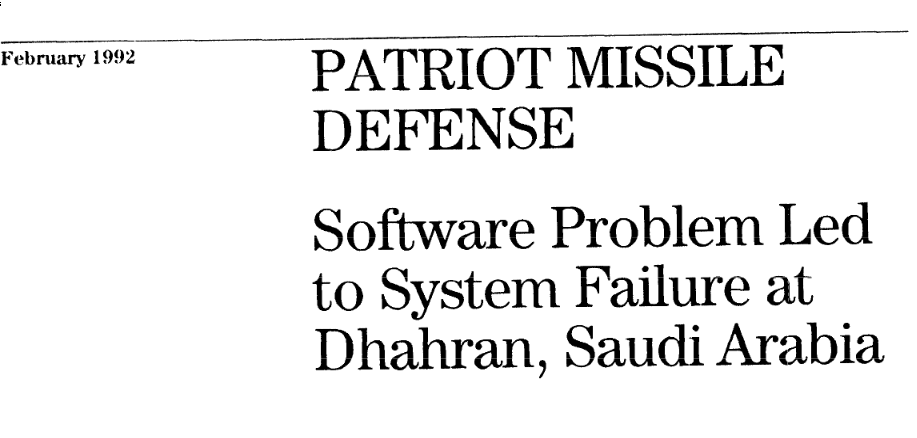
\includegraphics[width=0.5\textwidth]{material/us-govt-patriot-missile.png}}
     \end{frame}
}

\begin{frame}{Why abstract interpretation?}
There are other alternatives:
\begin{itemize}
\item ad-hoc, iterative DFA (not amenable to systematic correctness)
\item model checking (there is a neat connection with model checking)
\item type systems (limits choice of language, context-insensitive)
\end{itemize}
\end{frame}

\section{Lattices and order}
\begin{frame}{Lattices and Order Theory}
  \small
  \begin{columns}
  \begin{column}{0.5\textwidth}
  \begin{itemize}
  \item A lattice $(L, \sqcup, \sqcap, \sqsubseteq)$ is a partially ordered set (poset) with:
    \begin{itemize}
    \item a least upper bound (join) operation $\sqcup: L \times L \rightarrow L$
    \item and a greatest lower bound (meet) operation $\sqcap: L \times L \rightarrow L$
    \item $\sqcup, \sqcap$ determine the partial order $\sqsubseteq$
    \end{itemize}
  \item<9-> A bounded lattice has a least element $\bot$, (bottom)
    and greatest element $\top$ (top)
  \item<10-> Any powerset $\mathcal{P}(S)$ of a set $S$ is a bounded lattice where:
     $\top = S$,
     $\bot = \emptyset$,
     $\sqcup = \cup$,
     $\sqcap = \cap$,
     $\sqsubseteq = \subseteq$
  \end{itemize}
  \end{column}
  \begin{column}{0.5\textwidth}
    \vspace{-3cm}
  \begin{figure}[t]
    \centering
    \begin{tikzpicture}[x=2cm, y=1.5cm]
      \node(top)at (1,3){$\textcolor<9>{magenta}{\{+,-,0\} = \top}$} ;
      \node(pm)at (1,2){$\{+,-\}$} ;
      \node(mz)at (2,2){$\{-,0\}$} ;
      \node(pz)at (0,2){$\textcolor<4>{magenta}{\{+,0\}}$} ;
      \node(p)at (0,1){$\{+\}$} ;
      \node(m)at (2,1){$\{-\}$} ;
      \node(z)at (1,1){$\textcolor<8>{magenta}{\{0\}}$} ;
      \node(bot)at (1,0){$\textcolor<9>{magenta}{\emptyset = \bot}$} ;
      \draw(top)--(pm);
      \draw(top)--(mz);
      \draw(top)--(pz);
      \draw(pm)--(p);
      \draw(pm)--(m);
      \draw(mz)--(m);
      \draw[onslide={<7-8> draw=magenta, line width=1.2pt}](mz)--(z);
      \draw[onslide={<2-4> draw=magenta, line width=1.2pt}](pz)--(p);
      \draw[onslide={<3-4,6-8> draw=magenta, line width=1.2pt}](pz)--(z);
      \draw(p)--(bot);
      \draw(m)--(bot);
      \draw(z)--(bot);
    \end{tikzpicture}
    \caption{Hasse diagram of a sign lattice, built from the powerset of the set $\{+,-,0\}$}
  \end{figure}
  % \only<4>{\begin{figure}[t]
  %   \centering
  %   \begin{tikzpicture}[x=1.25cm, y=1.25cm]
  %     \node(top)at (0,1){$\top$} ;
  %     \node(e)at (-1,0){$e$} ;
  %     \node(o)at (1,0){$o$} ;
  %     \node(bot)at (0,-1){$\bot$} ;
  %     \draw(top)--(o)--(bot);
  %     \draw(top)--(e)--(bot);
  %   \end{tikzpicture}
  %   \caption{Hasse diagram of an even/odd lattice}
  % \end{figure}}
  \end{column}
  \end{columns}
\end{frame}

\begin{frame}{Relating lattices}
  \begin{columns}
    \begin{column}{0.6\textwidth}
      \small
      %\vspace*{-.75em}
    \begin{itemize}
    \item There is a relationship between the domain $EvenOdd$ and
      $\mathcal{P}(\mathbb{Z})$
    \item $\gamma : EvenOdd \to \mathcal{P}(\mathbb{Z})$,
      $\alpha : \mathcal{P}(\mathbb{Z}) \to EvenOdd$
      \begin{itemize}
      \item<2-> $\gamma(\top) = \mathbb{Z}, \gamma(\bot) = \emptyset$
      \item<2->
        $\gamma(o) = \{z \in \mathbb{Z} \mid z \text{ odd} \}$,
        $\gamma(e) = \{z \in \mathbb{Z} \mid z \text{ even} \}$
      \item<3-> $\alpha(S) = \bigsqcup\limits_{z \in S}
        \begin{cases}
          o & z \text{ odd}\\
          e & z \text{ even}
        \end{cases}
        $
      \end{itemize}
    \item<5-> $\alpha$ and $\gamma$ are kind of like inverses, though
      there is some information loss
    \item<6-> $\alpha$ happens to be the \emph{best possible} function to pair
      with $\gamma$ in a certain sense
      \begin{itemize}
      \item<7-> This relationship is known as a \emph{Galois Connection}
      \end{itemize}
    \end{itemize}
  \end{column}
  \begin{column}{0.4\textwidth}
    \begin{figure}
      \centering
      
      \vspace{-3cm}
      
      \begin{tikzpicture}[x=1.25cm, y=1.25cm]
        \node(top)at (0,1){$\top$} ;
        \node(e)at (-1,0){$e$} ;
        \node(o)at (1,0){$o$} ;
        \node(bot)at (0,-1){$\bot$} ;
        \draw(top)--(o)--(bot);
        \draw(top)--(e)--(bot);
      \end{tikzpicture}\\[0.5em]

      \onslide<4->{$\tikzmarkin<4>[above offset=0.4]{s}\alpha(5) + \alpha(-7) = e + o = o\tikzmarkend{s}$}
      \caption{Hasse diagram of an even/odd lattice ($EvenOdd$), and
        an example of abstracting an operator}
    \end{figure}
  \end{column}
  \end{columns}
\end{frame}

\begin{frame}{Galois Connections}
  \[ \textcolor<2->{gray}{\forall c \in \mathit{Concrete}, a \in \mathit{Abstract}.\, c \subseteq \gamma(a) \iff \alpha(c) \sqsubseteq a} \]
  \pause
  or, equivalently,
  $$ \tikzmark{ma}\textcolor<1,7->{gray}{\alpha, \gamma \text{ monotone}}\tikzmark{mb} \qquad \tikzmark{a}\textcolor<1,4-6,10->{gray}{c \subseteq \gamma(\alpha(c))}\tikzmark{b} \qquad \tikzmark{ra}\textcolor<1,4-9>{gray}{\alpha(\gamma(a)) \sqsubseteq a\tikzmark{rb}} $$
  \pause
  \vspace*{-1em}
  \begin{tightcenter}
   \begin{tikzpicture}
     \draw[fill=lightblue] (0,0.25) ellipse (1.75cm and 1.75cm);
     \node at (0,2.33) {$\mathcal{P}(\mathbb{Z})$};
     \node at (5.5,1.5) {$EvenOdd$};

     \node(top)at (5.5,1){$\top$} ;
     \node(e)at (4.5,0){$e$} ;
     \node(o)at (6.5,0){$o$} ;
     \node(bot)at (5.5,-1){$\bot$} ;
     \draw(top)--(o)--(bot);
     \draw(top)--(e)--(bot);

     \node (z) at (0,1.75) {$\mathbb{Z}$};
     \node (evens) at (-.75,1) {$evens$};
     \node (odds) at (.75,1) {$odds$};
     \node (two) at (0,-0.5) {$\{ 2 \}$};
     \node (empty) at (0,-1.0) {$\emptyset$};

     \draw<6,8-9>[->] (two) to [bend right] node [midway, below] {$\alpha$} (e) ;
     \draw<5-6>[->] (empty) to [bend right] node [pos=0.6, above] {$\alpha$} (bot) ;
     \draw<9,11->[->] (e) to [bend right] node [midway, above] {$\gamma$} (evens);
     \draw<12->[->] (evens) to [bend right] node [pos=0.6, above] {$\alpha$} (e);
     
   \end{tikzpicture}
 \end{tightcenter}

 \begin{tikzpicture}[overlay, remember picture]
   \draw<7-9>[draw=magenta, line width=1.1pt] ($(a)+(-.1em,-.4em)$) rectangle ($(b)+(0.1em,1em)$);
   \draw<7-9>[draw opacity=0] (a) to node [midway, below, yshift=-.5em] {$\alpha$ is sound} (b);
   \draw<4-6>[draw=magenta, line width=1.1pt] ($(ma)+(-.1em,-.4em)$) rectangle ($(mb)+(0.1em,1em)$);
   %\draw<4>[draw opacity=0] (ma) to node [midway, below, yshift=-.5em] {$\alpha$ is sound} (mb);
   \draw<10-12>[draw=magenta, line width=1.1pt] ($(ra)+(-.1em,-.4em)$) rectangle ($(rb)+(0.1em,1em)$);
   %\draw<11>[draw opacity=0] (ra) to node [midway, below, yshift=-.5em] {$\alpha$ is sound} (rb);
 \end{tikzpicture}
\end{frame}

\section{Abstract interpretation}
\begin{frame}{Abstract interpretation}
  \begin{itemize}
  \item<1-> Introduced by Cousot and Cousot in 1977 for a flow-chart language \footcite{cousot1977abstract}
  \item<2-> Deep connections to math, correct by construction \footcite{cousot1979systematic}
  \item<3-> Expanded to be used in different kinds of semantics \footcite{schmidt1998trace,schmidt2009abstract}
  \item<4-> General idea: Create an \emph{abstract} interpreter that
    overapproximates the \emph{concrete} interpreter's behavior
    soundly.
  \end{itemize}
\end{frame}

\section{Predicate abstraction \& Abstraction Refinement}
\subsection{Predicate abstraction}
\subsection{Abstraction refinement}

\section{Static analysis of control software}
\begin{frame}{What is control software?}
  Example: autopilots, nuclear plant rod controller etc.
  
  \begin{itemize}
  \item<2-> Has multiple synchronous components
    \begin{itemize}
    \item<3-> Control part of the state is not as straightforward as sequential programs
    \end{itemize}
  \item<4-> Variables with complex numeric relationships
  \end{itemize}
\end{frame}
\subsection{Dynamic state partitioning}
\begin{frame}{\todo{Bultan et al. \& cite Jeannet}}
  
\end{frame}

\begin{frame}{\todo{Chen \& Cousot}}
  
\end{frame}

\subsection{Combination of domains}
\begin{frame}{A plethora of domains}
  \footnotesize
  \begin{tabular*}{1.0\linewidth}{lcc}
    \textbf{Domain & Constraints & Complexity} \\
    % Presburger formulas\footcite{bultan_model-checking_1999} & Presburger arithmetic & $ \bigO(2^{2^{2^{pn}}}) $ \\
    Polyhedra\footcite{cousot1978automatic} & \( \sum_{j} c_{ij}x_j \leq 0 \) & $ \bigO(2^n) $ \\
    Octagons\footcite{mine2004weakly} & \( \pm x \pm y \leq c \) & $ \bigO(n^3) $ \\
    Pentagons\footcite{logozzo2010pentagons} & \( x \in [a,b] \wedge x < y \) & $ \bigO(n^2) $ \\
    % Gauges\footcite{venet2012gauge} & \( x \in \left[\sum_{j} a_{j}\lambda_j, \sum_{j} b_{ij}\lambda_j \right] \) & $ \bigO(n2^l) $ \\
    Arithmetic-geometric progressions\footcite{feret2005arithmetic} & \( x \mapsto ax + b \) & $ \bigO(n) $
  \end{tabular*}

  \uncover<1->{Also: congruences, floating-point variants\footcite{mine2004relational}, gauges\footcite{venet2012gauge} \ldots{}} \\
  \uncover<2->{\alert{How do we choose/combine them?}}

  \vspace{1em}
\end{frame}

\begin{frame}{Reduced products}
  \todo{Null \& cycle example}
\end{frame}

\begin{frame}{Sharing information}
  \todo{Add an example that gets refined as we communicate the info}
\end{frame}

\begin{frame}{Variable packing}
  \todo{Explain with an example}
\end{frame}

\begin{frame}{Binary product abstract domain functor}
  \todo{$\times : \mathcal{D \times D} \rightarrow \mathcal{D}$}

  \todo{Add the functor from ASTRÉE}
\end{frame}

\begin{frame}{Reduced products \& combination of DP}
  \todo{\footcite{cousot2011reduced}}
\end{frame}

\section{Memes}
\begin{frame}{\todo{Memes}}\end{frame}

\begin{frame}[standout]
  Thank you!
\end{frame}

\appendix

\begin{frame}{Dependent object types}
  
\end{frame}
\end{document}

%%% Local Variables:
%%% mode: latex
%%% TeX-master: t
%%% TeX-engine: xetex
%%% End:
